\documentclass[a4paper]{article}
\usepackage{hyperxmp}
\usepackage{titling}
\usepackage[colorlinks,linkcolor=blue]{hyperref}
\usepackage{graphicx}
\usepackage{fancyhdr}
\usepackage{a4wide}
\usepackage{xspace}
\usepackage{lastpage}
\usepackage{tikz}

\makeatletter
\newcommand*{\rom}[1]{\expandafter\@slowromancap\romannumeral #1@\xspace}
\makeatother

\newcommand{\myhref}[2]{{\href{#1}{\textcolor{blue}{#2}}}}
\fancyhead[L]{\thetitle}
\fancyhead[R]{\it\thepage\ of \pageref{LastPage}}
\fancyfoot[C]{\centerline{\small \copyright\ \theauthor, 2013. This work is licensed under a \myhref{http://creativecommons.org/licenses/by-sa/3.0/}{Creative Commons Attribution-ShareAlike 3.0 Unported License.}}}
\pagestyle{fancy}

%% PDF meta-data
\hypersetup{%
pdftitle={Assigment 1 for the course on city design. Ideas and Forces That Have Shaped Your City},
pdfauthor={Vitaly Repin},
pdfcopyright={This work is licensed under a Creative Commons Attribution-ShareAlike 3.0 Unported License},
pdfsubject={Designing City},
pdfkeywords={design,city,map},
pdflicenseurl={http://creativecommons.org/licenses/by-sa/3.0/},
pdfcaptionwriter={Vitaly Repin},
pdfcontactcity={Espoo},
pdfcontactcountry={Finland},
pdfcontactemail={vitaly.repin@gmail.com},
pdflang={en}
}

%% City name
\newcommand{\mycity}{Espoo\xspace}
%% Author
\author{Vitaly Repin}
%% Title
\title{Ideas and Forces That Have Shaped My City: \emph{\mycity}}

\date{October, 2013}

\begin{document}
%% Environment to draw maps
\newenvironment{mymap}[1]{%
\begin{tikzpicture}
%% Change scale size to suit your needs
\node[anchor=south west,inner sep=0] (image) at (0,0) {\includegraphics[keepaspectratio,width=\textwidth]{#1}};
\begin{scope}[x={(image.south east)},y={(image.north west)}]
}{
\end{scope}
\end{tikzpicture}
}

\definecolor{myblue}{HTML}{0EBFE9}
%% Adapted from: http://tex.stackexchange.com/questions/7032/good-way-to-make-textcircled-numbers
%% Can be used only inzide tikzpicture environment
\newcommand{\circled}[2]{\node[shape=circle,draw,inner sep=2pt,fill=myblue] at (#1) {\textcolor{white}{#2}};}

%% Page 1: Map of the city in IXX century
\section{Map of \mycity in \rom{19} century}

\begin{mymap}{map1}
\circled{0.1,0.3}{1}
\circled{0.44,0.48}{2}
\circled{0.75,0.56}{3}
\end{mymap}
\centerline{Map of Espoo (Espoon keskus (city center) and Kauklahti areas) in 1855~\cite{espoo1855}.}

\newpage

%% Page 2: Map of the city in the mid-20th century,
\section{Map of \mycity in the mid-\rom{20} century}
\begin{mymap}{map2}
\circled{0.14,0.33}{1}
\circled{0.6,0.6}{2}
\circled{0.88,0.73}{3}
\end{mymap}
\centerline{Map of Espoo (Espoon keskus (city center) and Kauklahti areas) in 1945~\cite{espoo1945}.}

\newpage

%% Page 3: Map of the city today (screenshot from http://www.openstreetmap.org/
\section{Map of \mycity in the year of 2013}
%% Change scale size to suit your needs
\begin{mymap}{map3}
\circled{0.05,0.22}{1}
\circled{0.63,0.54}{2}
\circled{0.9,0.7}{3}
\end{mymap}
\centerline{Map of Espoo (Espoon keskus (city center) and Kauklahti areas) in 2013~\cite{espoo2013}.}

\newpage

%% Page 4: Photographs
\section{Photographs of \mycity}
\begin{tabular}{lp{.4\textwidth}}
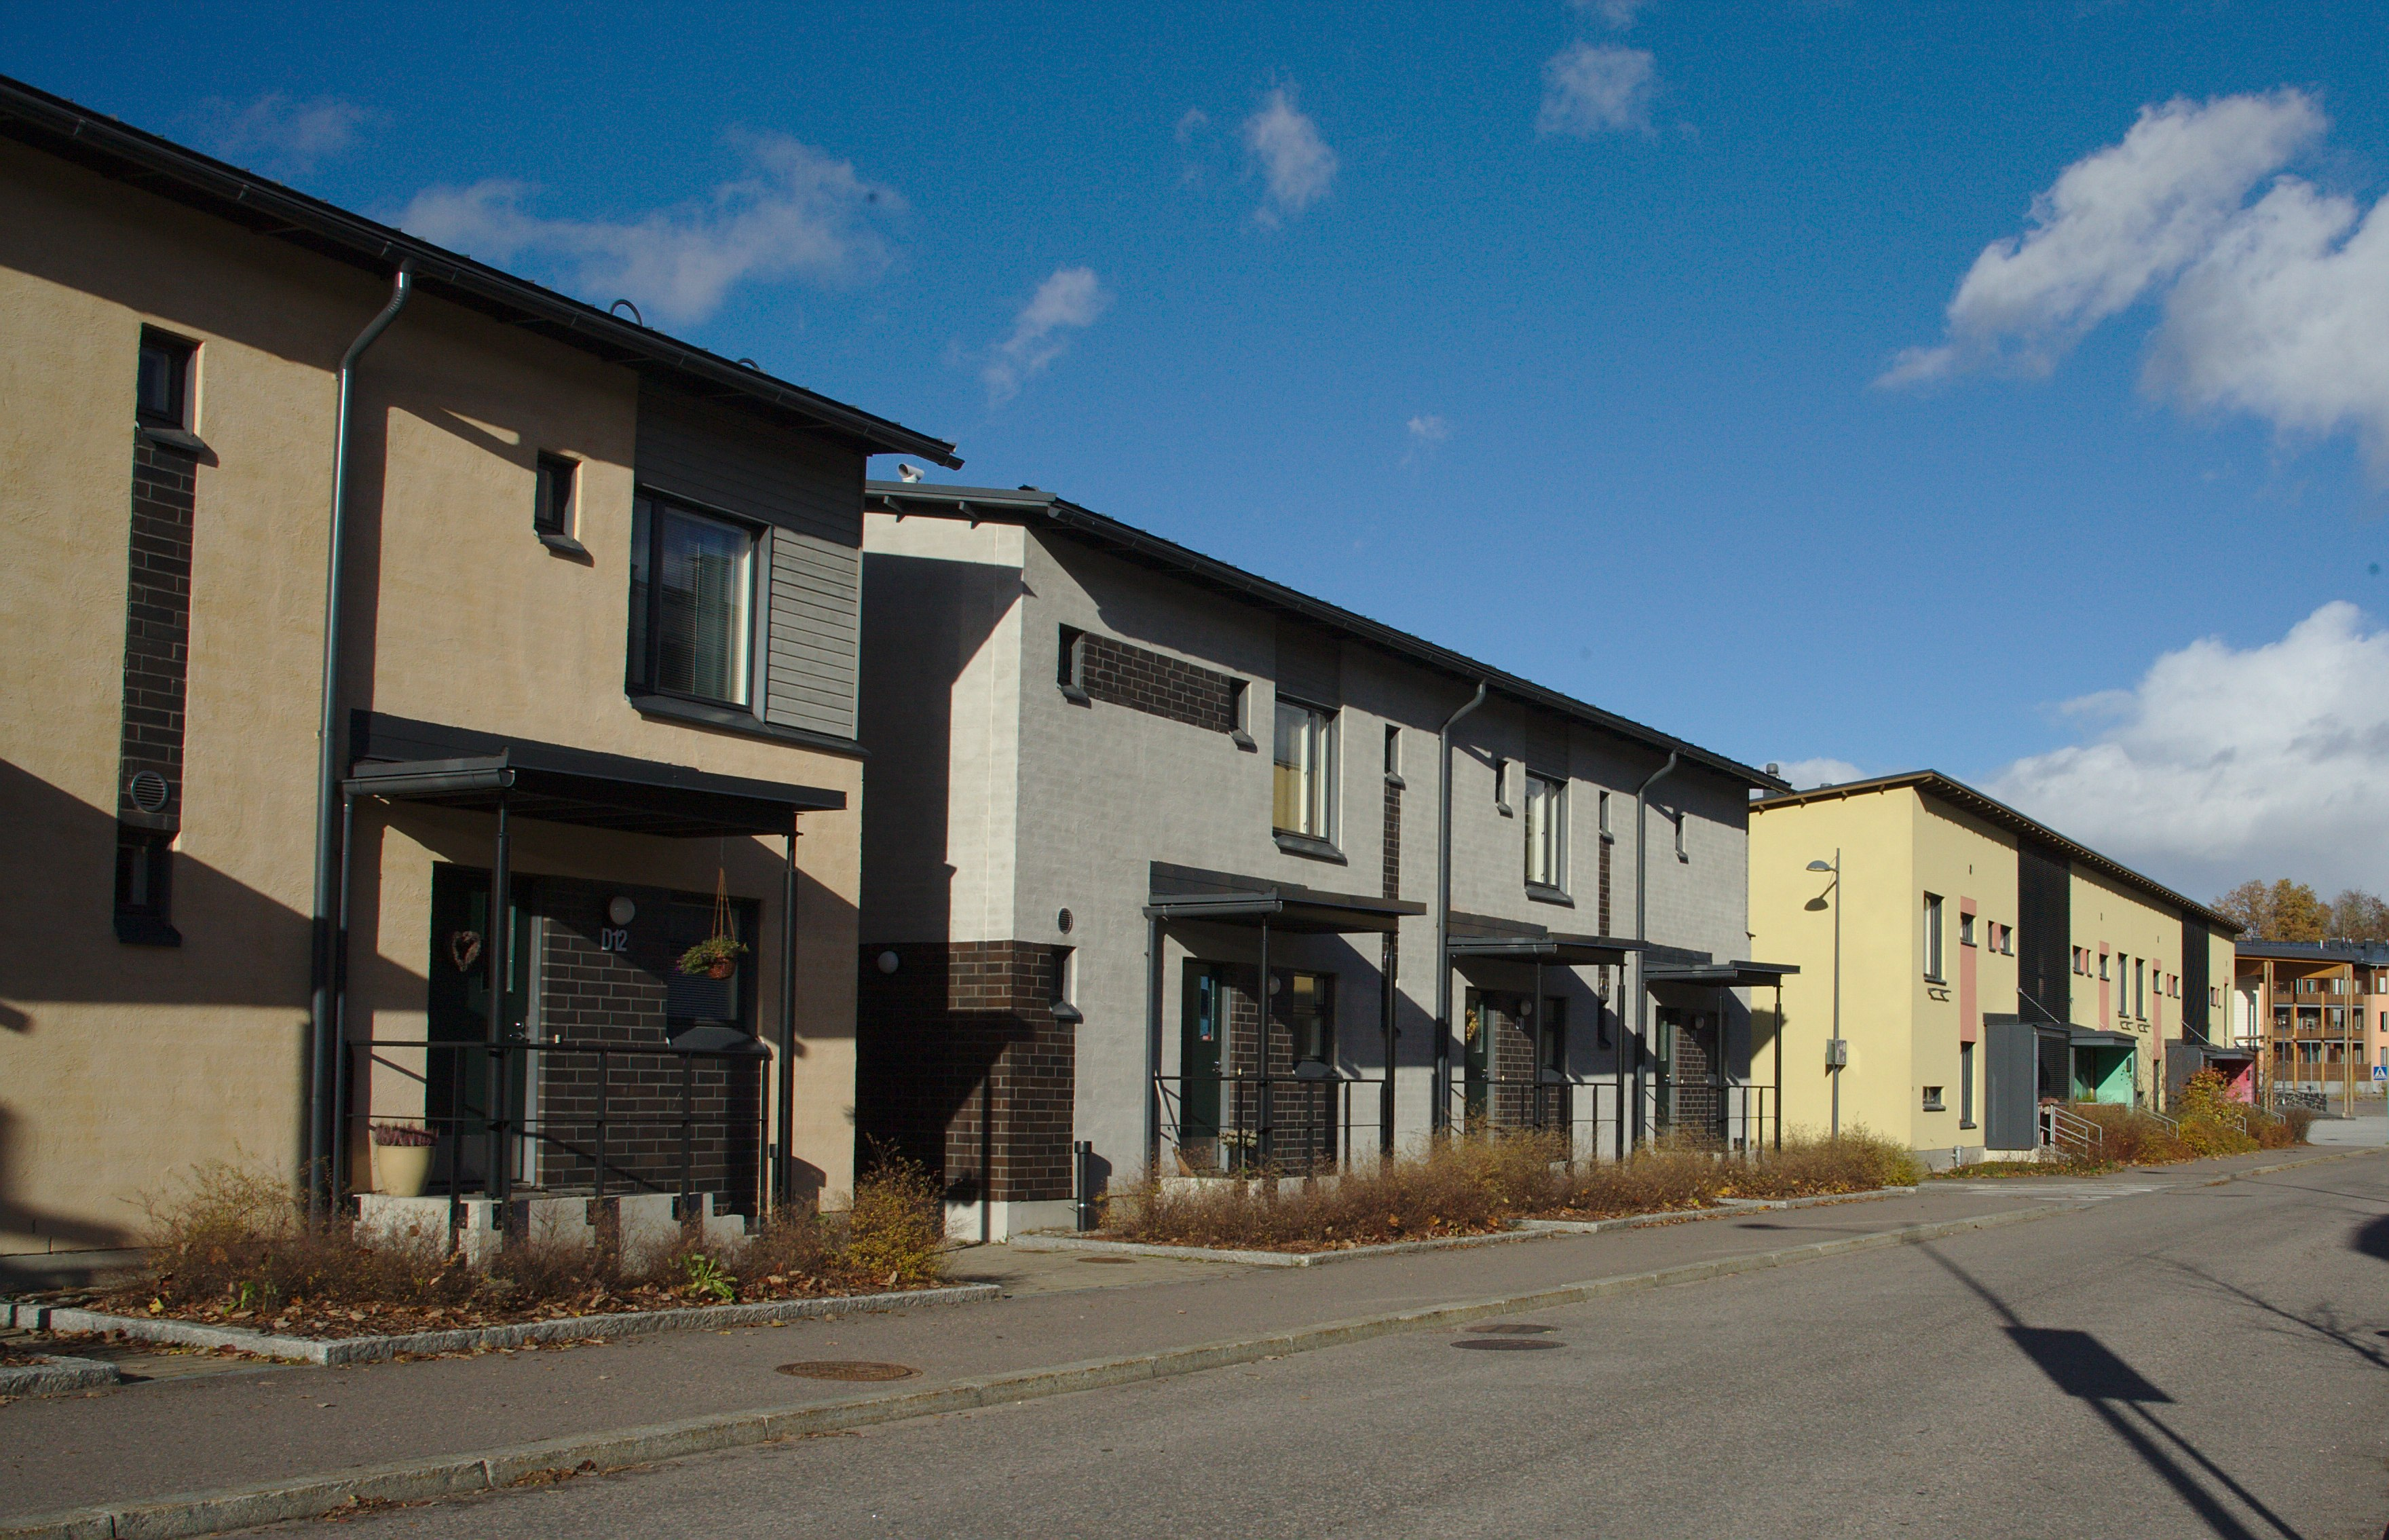
\includegraphics[keepaspectratio,width=.5\textwidth]{traditional} & Comments about photo1\\[.2cm]
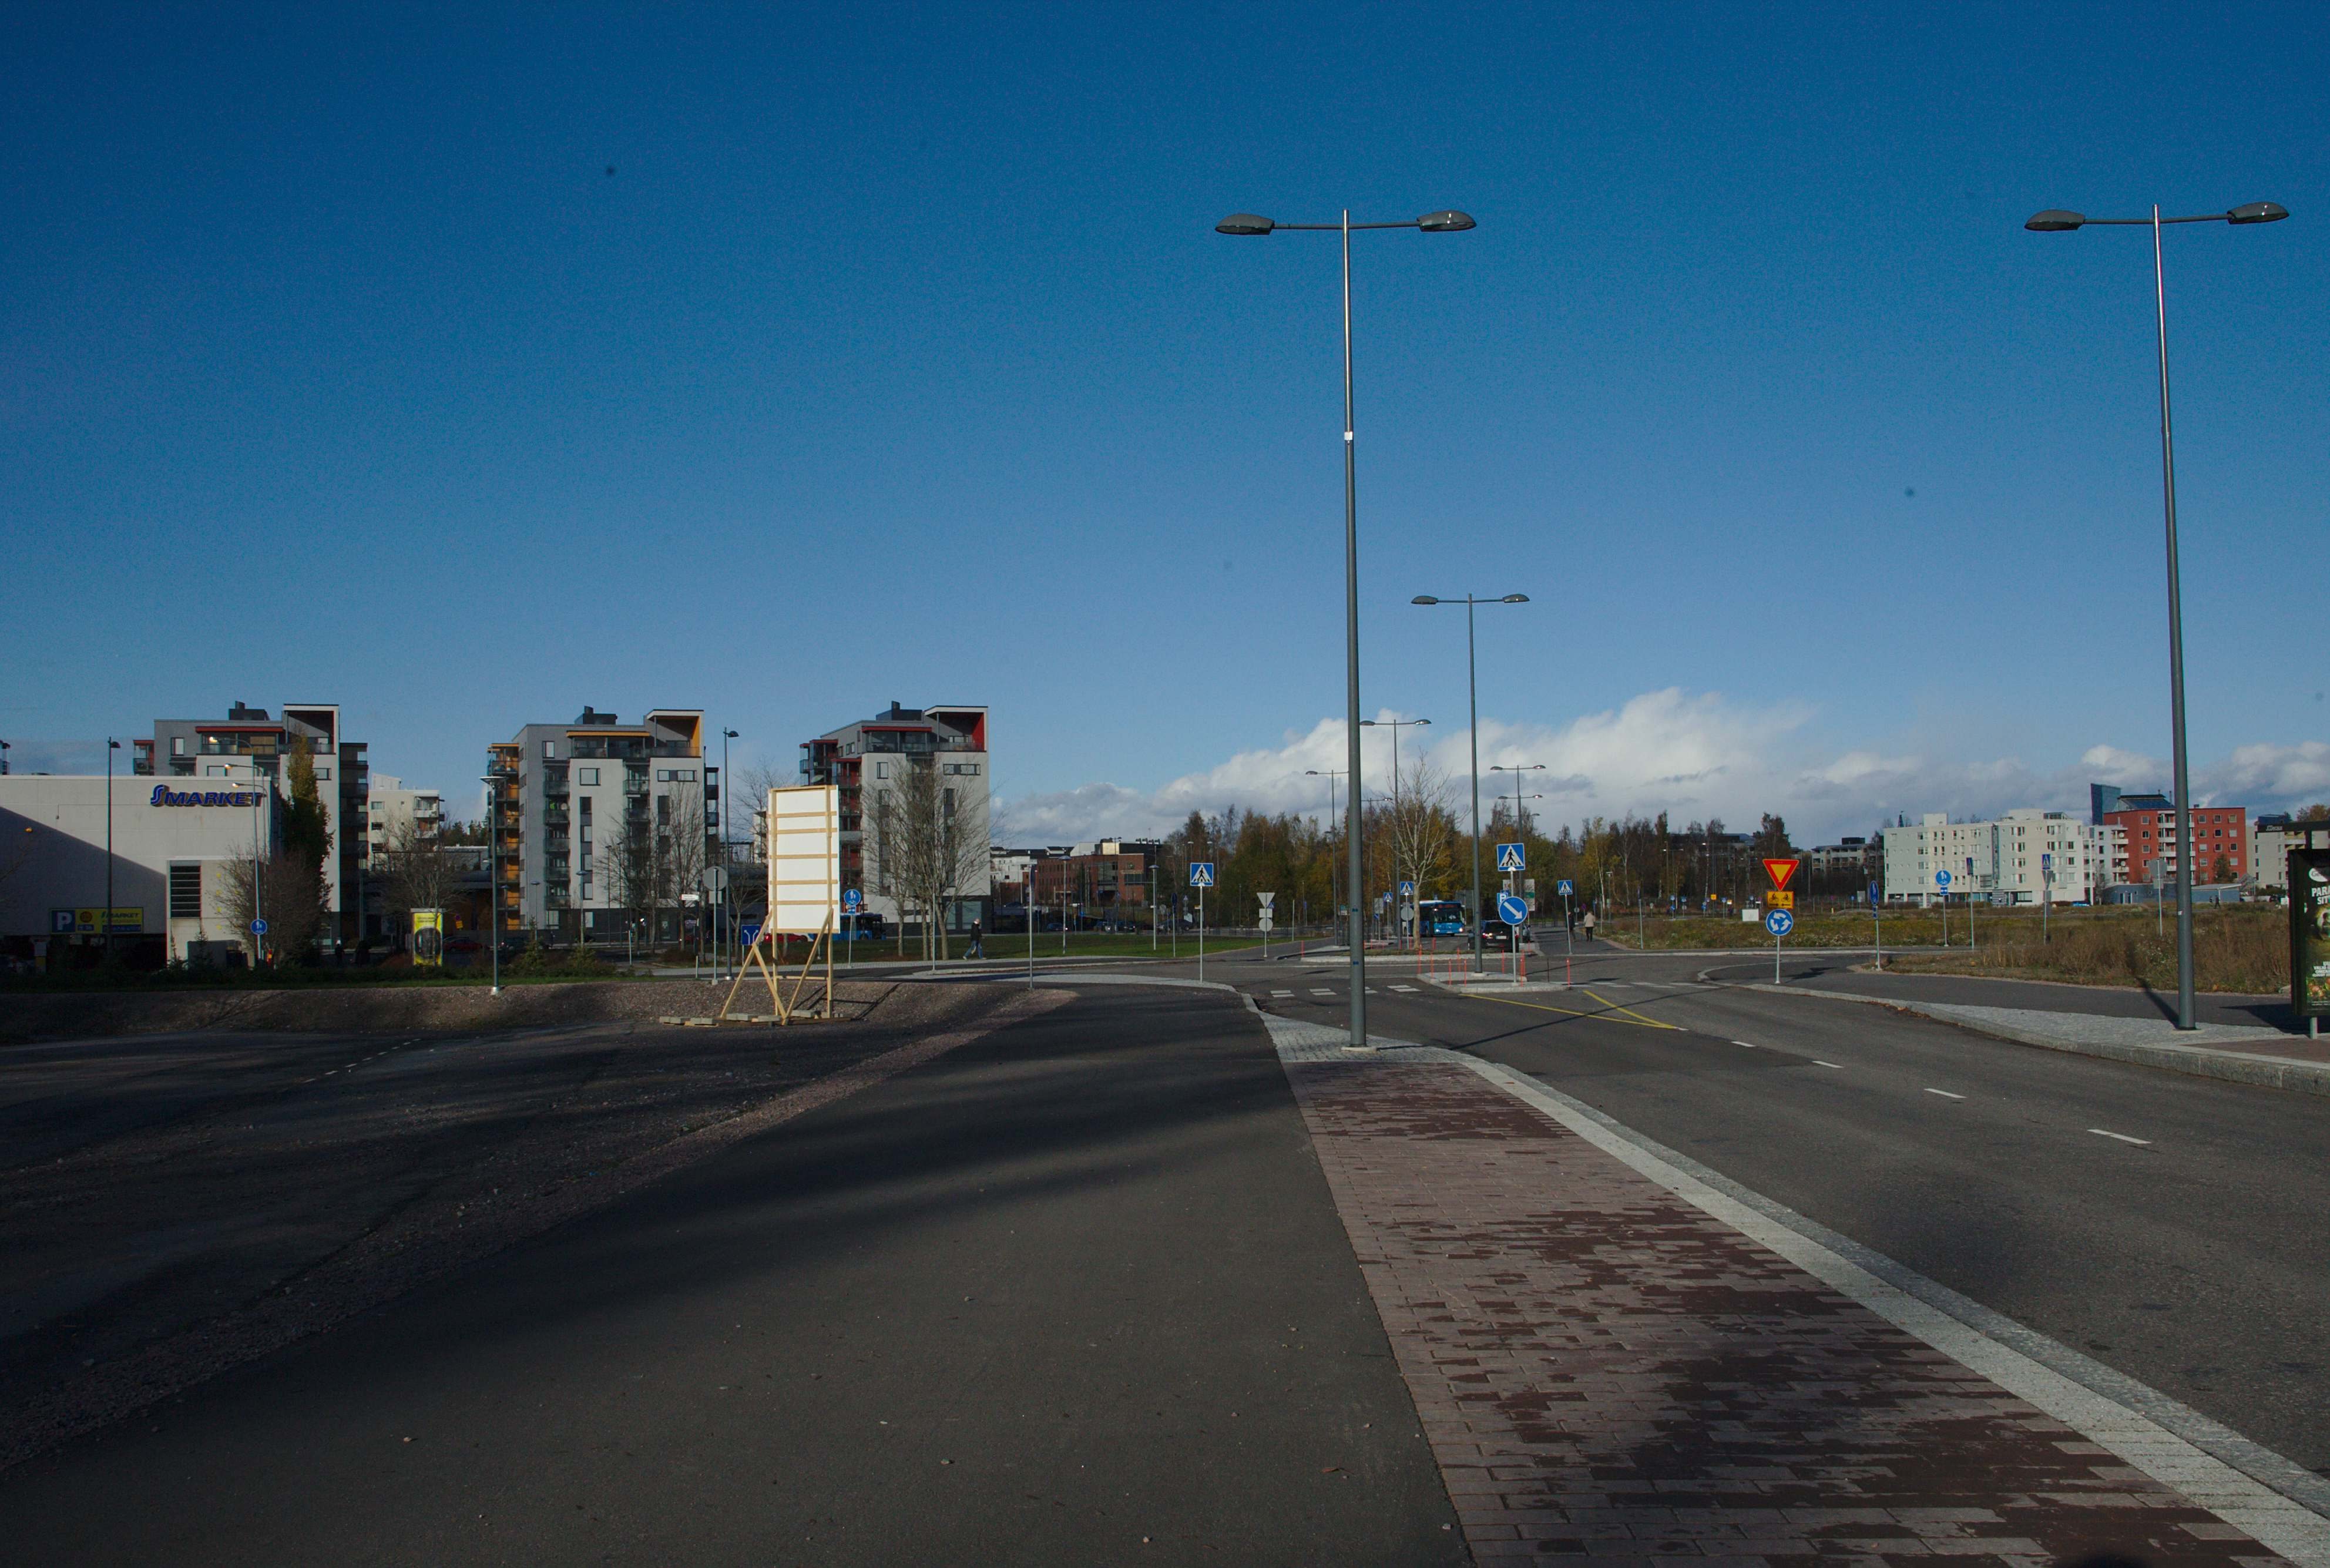
\includegraphics[keepaspectratio,width=.5\textwidth]{modern} & Comments about photo2\\[.2cm]
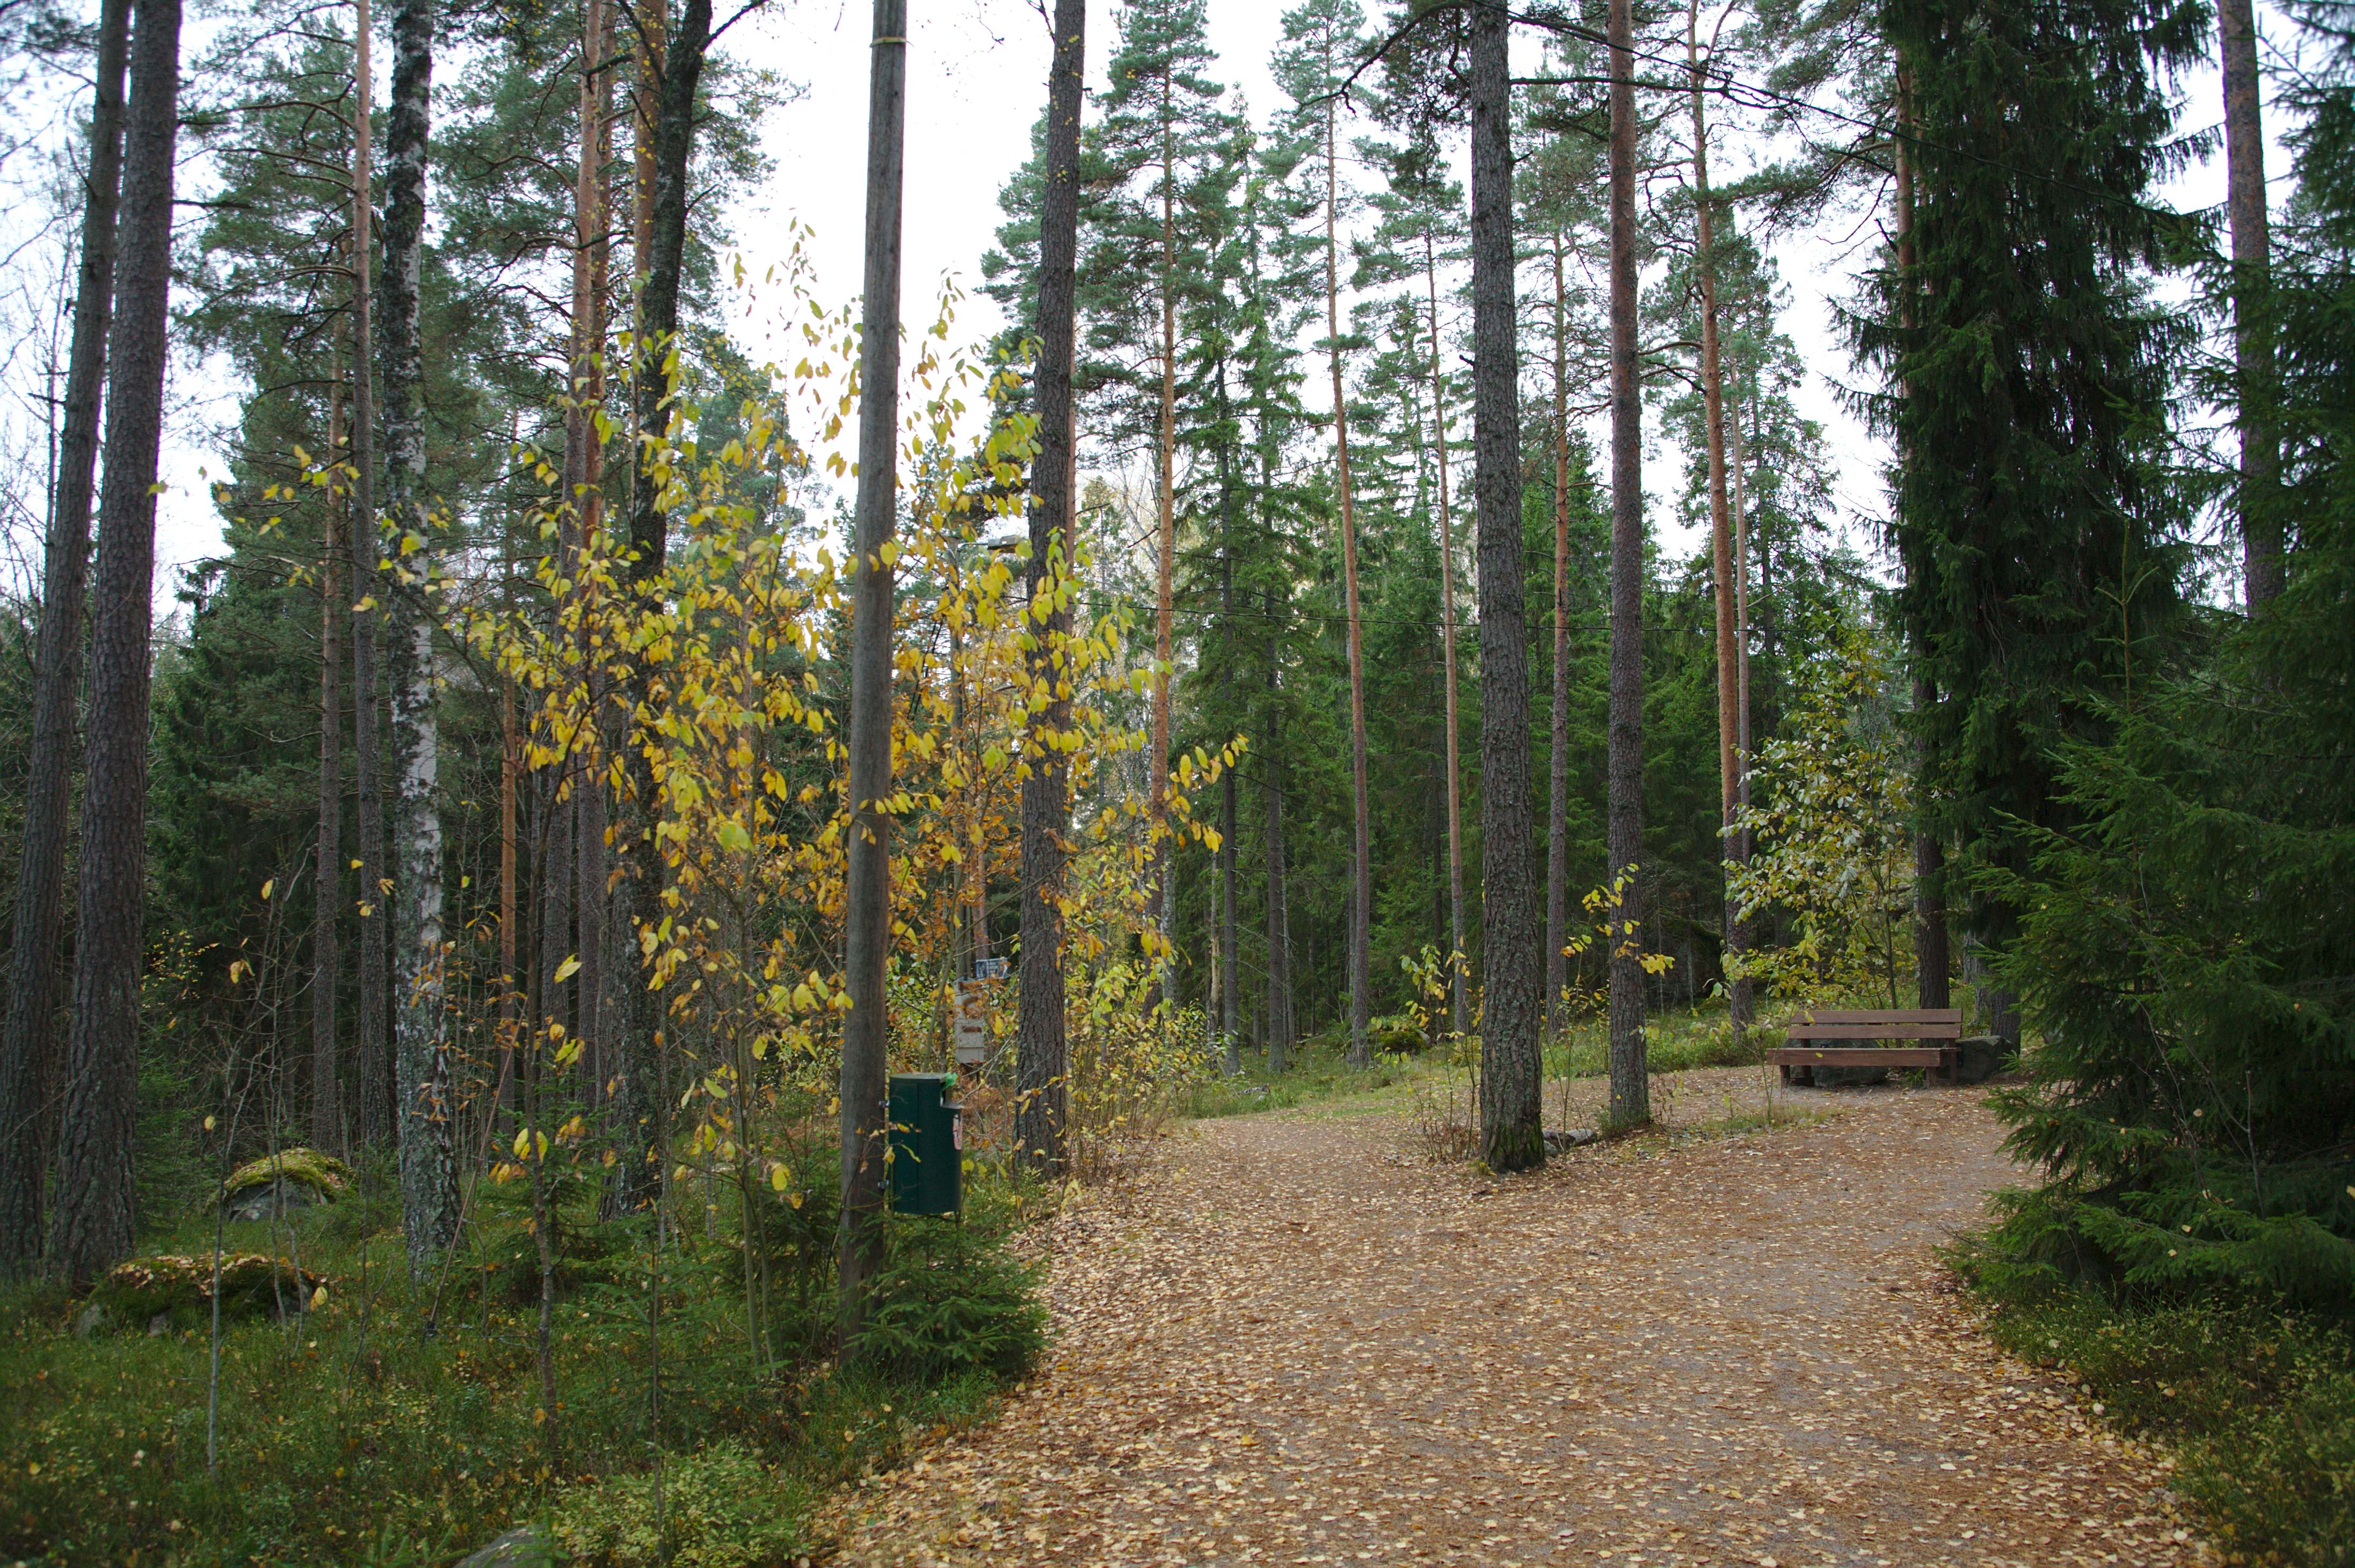
\includegraphics[keepaspectratio,width=.5\textwidth]{green} & Comments about photo3\\
\end{tabular}

\begin{thebibliography}{9}
\bibitem{espoo1855} \myhref{http://www.vanhakartta.fi/historialliset-kartat/kaupunkikartat/sekalaiset-kaupunkikartat/@@mapview?handle=hdl_123456789_6888}{Kalmbergin kartasto R VII : List 7. 1855.}
\bibitem{espoo1945} \myhref{http://koti.kapsi.fi/timomeriluoto/KARTAT/Topografiset\%20kartat/Topografinen\%20kartta\%201:20.000\%20Espoo\%201945.jpg}{Topografinen kartta 1:20.000 Espoo 1945.}
\bibitem{espoo2013} \myhref{http://www.openstreetmap.org/\#map=14/60.2034/24.6415}{OpenStreetMap. Espoo. 2013}
\end{thebibliography}
\end{document}
